\section{Durchführung}
\label{sec:Durchführung}
Der Versuch wird auf einer vorgefertigten Platine durchgeführt. Der gesamte Aufbau
ist in Abbildung \ref{fig:aufbau} zu sehen.

\begin{figure}
  \centering
  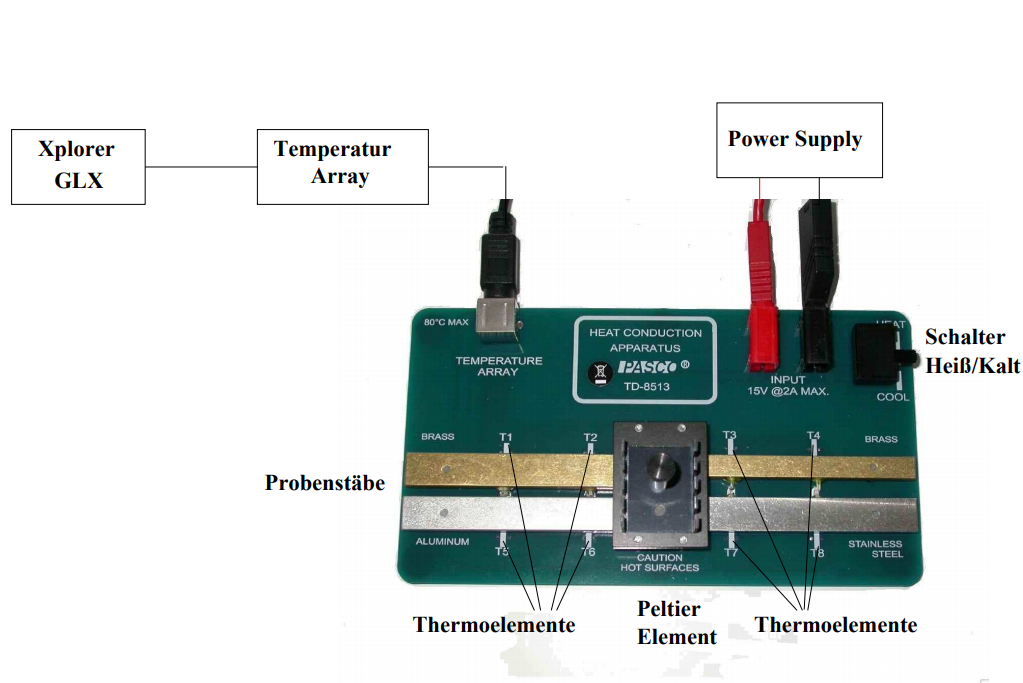
\includegraphics[width=300pt]{data/aufbau.png}
  \caption{Versuchsaufbau und Darstellung der Aufnahme der Daten \cite{Versuchsanleitung}}
  \label{fig:aufbau}
\end{figure}

Die zu untersuchenden Materialien liegen als vier rechteckige Stäbe auf der Platine vor,
je ein Stab besteht aus Aluminium und aus Edelstahl und zwei Stäbe mit unterschiedlich
großer Querschnittsfläche bestehen aus Messing. Mittig angebracht ist ein Peltier-Element,
mit dem je nach Einstellung des Schalters oben rechts entweder ein Kühlen oder
Erwärmen der Stäbe von der Mitte aus möglich ist. Die maximal zulässige Spannung am Peltier-Element beträgt $\SI{15}{\volt}$.
An jedem der Stäbe sind zwei Thermoelemente angebracht, die mit T1 bis T8 bezeichnet werden
\footnote{Im Folgenden seien auch die Temperaturen an den entsprechenden Thermoelementen ungenau mit T1 bis T8 bezeichnet.}.
Mit diesen ist die Messung der Temperatur der Stäbe an den Stellen möglich,
an denen sie angebracht sind. Die Daten der Messung werden an den Xplorer GLX, einen Datenlogger, weitergegeben.
Während jeglicher Messungen wird eine Wärmeisolierung über die Stäbe gelegt, um
den Austausch von Wärme mit der Umgebung zu minimieren. Nach Beendigung jeder Messung
wird die Wärmeisolierung entfernt und die Stäbe werden gekühlt.

Am Datenlogger wird überprüft, ob alle acht Temperaturen gemessen und angezeigt werden.
Die Abtastrate wird auf $\SI{10}{\second}$ eingestellt.
Es wird der Abstand $x$ zwischen den Thermoelementen gemessen.

Zur Untersuchung der Wärmeleitung und Wärmeleitfähigkeit der Stäbe werden zwei
verschiedene Methoden angewandt.

\subsection{Statische Methode}
\label{sec:statische methode}
Bei dieser Methode werden die Stäbe während der Messung durchgehend erwärmt. Die
am Peltier-Element anliegende Spannung wird auf ungefähr $\SI{12.2}{\volt}$
geregelt, sodass ein Strom einer Stärke von circa $\SI{1}{\ampere}$ anliegt. Der Schalter wird
auf Heizen gestellt und die Messung an allen acht Thermoelementen durchgeführt, bis
T7 45 Grad Celsius beträgt. Dieses ist gerade das nahe Thermoelement am Edelstahlstab.
Die Messdaten an den fernen Thermoelementen werden in einem Temperatur-Zeit-Diagramm dargestellt.
T1 und T4, sowie T5 und T8 werden dabei jeweils in einem Diagramm aufgetragen.
Außerdem werden Diagramme für die Temperaturdifferenzen $T7 - T8$ und $T2 - T1$
angefertigt. Die Graphiken werden vor Ort ausgedruckt.

\subsection{Dynamische Methode}
\label{sec:dynamische methode}
Die Stäbe werden bei der Durchführung dieser Methode periodisch gewärmt und gekühlt.
Die Abtastrate wird auf $\SI{2}{\second}$ eingestellt. Als Spannung wird circa
$\SI{5.2}{\volt}$ eingestellt. Die anliegende Stromstärke beträgt dann ungefähr $\SI{0.7}{\ampere}$.
Nach der Überprüfung, ob die
Stäbe ausreichend abgekühlt sind, wird die Messung begonnen. Die Periodendauer beträgt
dabei $\SI{80}{\second}$, auf $\SI{40}{\second}$ Heizen folgt also $\SI{40}{\second}$ Kühlen
und so weiter. Nach zehn Perioden wird die Messung beendet. Es wird ein Diagramm
der Temperaturen T1 und T2 am breiten Messingstab erstellt und gedruckt, dies wird
für die Temperaturen T5 und T6 am Aluminiumstab wiederholt.

Sobald die Stäbe wieder hinreichend abgekühlt sind, wird die zweite Messung der
dynamischen Methode begonnen. Diese wird analog zur ersten durchgeführt, nur wird
mit einer Periodendauer von $\SI{200}{\second}$ gewärmt und gekühlt.
Wieder wird nach zehn Perioden die Messung beendet. Ein Diagramm der Temperaturen T7 und T8
am Edelstahlstab wird ausgedruckt.
